\documentclass[11pt]{article}
\usepackage[margin=1in]{geometry}
\usepackage{amsmath,amssymb}
\usepackage{booktabs}
\usepackage{graphicx}
\usepackage{float}
\usepackage{caption}
\usepackage{threeparttable}
\usepackage{siunitx}
\usepackage{url}
\usepackage{hyperref}
\usepackage{xcolor}
% group-digits=integer is essential: siunitx v3 groups the DECIMAL part by default, which
% renders 0.0349 as "0.034,9" in every S column.
\sisetup{table-number-alignment=center, detect-weight=true,
         group-separator={,}, group-minimum-digits=4, group-digits=integer}
\captionsetup{font=small,labelfont=bf}
\captionsetup[table]{skip=4pt}
\hypersetup{colorlinks=true,linkcolor=blue!45!black,urlcolor=blue!45!black,
            citecolor=blue!45!black}
% long file paths cannot hyphenate; let them break after / and _ instead
\newcommand{\code}[1]{\texttt{\small\begingroup\hyphenpenalty=10000 #1\endgroup}}
\emergencystretch=3em
\sloppy

\title{\textbf{What PE-RankFormer is and is not better at}\\[0.35em]
\large A re-evaluation of prime-editing pegRNA ranking against a\\
mechanistic baseline, on a reserved external panel}
\author{}
\date{10 September 2026}

\begin{document}
\maketitle

\noindent\textbf{Scope update, 10 September 2026.} The analysis below records the
source-only E01--E24 programme. The current research summary is
\path{explore_v2/SUMMARY_REPORT.md}; E25--E32 are incorporated in
\href{adaptation_report.pdf}{the updated adaptation report}.
Target-library adaptation now exceeds released OptiPrime on held-out loci within
this library, but this does not alter the zero-shot comparison below. The later
audit withdraws claims of low-budget harm, four-fold deployed-selector retention,
and wholesale rejection of specialized losses or dual heads. Those claims must
not be inferred from historical descriptions of the research programme.
\medskip

\begin{abstract}
\noindent
PE-RankFormer was reported to rank prime-editing pegRNAs better than OptiPrime, a
mechanistic reaction model, by $+0.0389$ pooled Spearman on a held-out fold. This report
re-examines that claim on a second surface and under the estimand a user actually faces, and
reaches a split verdict. The correlation claim \emph{replicates}: on a 288{,}793-pegRNA
library absent from either model's training data, PE-RankFormer leads by $+0.0159$ Spearman
and $+0.0163$ calibrated Pearson, and a calibrator frozen on development data transfers to
the new library unchanged. A second, previously implicit claim does \emph{not} survive. When
the grouping is corrected to the deployment unit --- one canonical allele in one experimental
context, the thing a user has already fixed before choosing a pegRNA --- OptiPrime obtains
more efficiency from its single nominated design, by $0.00064$
(95\% CI $[0.00038, 0.00089]$), a deficit that widens with candidate depth. The two metrics
rank the same models in opposite order, and we reproduce the reversal inside our own
ablations. We size the disagreement against a perfect chooser: it is 2.6\% of the available
gain, with both models far closer to each other than either is to random selection. An
eight-arm, eighteen-run training matrix identifies \emph{batch composition}, not ranking-pair
supervision, as what pays, correcting a causal claim we had previously made. Re-scored on the
panel, batch composition alone recovers the entire gain over the released recipe
($+0.00141$) and draws level with the published model, while two components the development
fold had endorsed with three-of-three seed agreement reverse sign on the external
library. We diagnose the residual error as a conditional
preference for longer PBS and RTT, and show that a global length correction cannot remove it.
All numbers are generated from versioned JSON artifacts and checked by an automated
verifier.
\end{abstract}

\tableofcontents
\bigskip

% =====================================================================
\section{Why this re-evaluation was necessary}

A pegRNA-ranking model earns its keep at one moment: a user has decided which allele to
install, in which cell line, with which editor, and must pick one design from several
candidates. Everything upstream of that --- which locus is easy, which cell line edits well
--- is not the model's decision to make, because the user has already made it.

The original evaluation did not measure that moment. It grouped candidates by
\emph{protospacer} and reported a pooled rank correlation over all rows. Both choices admit
information the user does not have to predict. Pooled correlation over a heterogeneous corpus
is dominated by between-locus and between-context variance; a protospacer group mixes designs
that install different alleles under different conditions. A model can lead on that metric
while losing the decision, and we show below that this is exactly what happens.

This report re-runs the comparison under the deployment estimand, on a reserved external
surface, with tested endpoint code. Twenty-four experiments (E01--E24) are recorded in
\code{explore\_v2/}; each writes a JSON artifact beside its script, and
\code{explore\_v2/verify\_report.py} re-checks recorded numeric claims against those artifacts.
Endpoint invariants are pinned by 13 unit tests.

% =====================================================================
\section{The estimand, and how the grouping was fixed}

\subsection{Canonical allele keys}

The decision unit is one \emph{canonical allele} $\times$ one \emph{experimental context}.
Building it (\code{explore\_v2/canon.py}) requires more care than string equality on the edit
field:

\begin{itemize}\itemsep2pt
\item \textbf{Minimal edit.} Trim the common prefix and suffix so that
\code{AAG}$\rightarrow$\code{AAAG} and \code{AG}$\rightarrow$\code{AAG} are recognised as the
same insertion.
\item \textbf{Left-normalisation, in both orientations.} An indel in a homopolymer has many
equivalent representations; VCF-style left-normalisation picks one. This must be applied
\emph{independently on each strand}, not applied once and reverse-complemented --- a bug we
made and fixed, which affected 61.7\% of 51{,}012 indel pairs (\S\ref{sec:corrections}).
\item \textbf{Strand normalisation} and \textbf{12\,bp flanks} read off the site's longest
observed window, so the same allele reported in two library designs with different window
lengths keys identically.
\end{itemize}

Context is the tuple \{source study, cell type, PE type, Cas9 type, PAM, PEmax, MLH1dn, NRCH,
time\}; design is \{spacer, PBS, RTT, motif, scaffold, linker, epegRNA\}. A candidate is one
distinct design; repeated measurements of the same design are averaged before ranking.

\subsection{What regrouping reveals}

\begin{table}[htbp]\centering\footnotesize
\caption{The evaluation population changes when the grouping is corrected (fold 0).}
\label{tab:grouping}
\begin{tabular}{l S[table-format=4.0] S[table-format=4.0]}
\toprule
& {Protospacer grouping} & {Allele $\times$ context} \\
\midrule
Groups with $\geq 2$ distinct designs & 670 & 1463 \\
Groups with $\geq 3$ distinct designs & {--} & 85 \\
Groups with $\geq 5$ distinct designs & 146 & 0 \\
\bottomrule
\end{tabular}
\end{table}

Two consequences follow. First, the population the original evaluation described --- 735
``targets with five or more designs'' --- counts five or more \emph{rows}, not designs; the
median number of distinct designs in those groups is two. Second, under the correct grouping
fold 0 contains \emph{no} group with five candidates, so a ``best of five'' endpoint cannot be
computed on it at all. This is the concrete reason an external panel was required.

\subsection{Four endpoint defects}

Re-implementing the endpoints in a tested module (\code{explore\_v2/endpoints.py}) surfaced
four defects in the original scoring, each of which flatters or distorts a comparison:

\begin{enumerate}\itemsep2pt
\item candidates were counted as \emph{rows}, so a design measured three times counted three
times toward group depth;
\item achieved efficiency at $k$ was averaged over groups shallower than $k$, where it is
undefined;
\item the random-choice hit rate ignored tied measured maxima, understating the baseline
(0.3354 against a correct 0.4442);
\item the paired bootstrap returned $p \approx 0$ for a degenerate all-zero difference.
\end{enumerate}

% =====================================================================
\section{The reserved panel}

Fold 0 cannot answer the deployment question, so we reserved a surface for comparative
evaluation, built from Kim's large variant library (288{,}793 pegRNAs), which is absent from OptiPrime's training mix --- that
mix took only \code{LibSmall}. The panel and its analysis were pre-registered
(\code{explore\_v2/PREREGISTRATION\_reserved\_panel.md}) and unblinded once, for one
confirmatory comparison. Every later use of the panel in this report is development work and
is labelled as such in the artifact that reports it; component decisions taken from those uses
would need a freshly reserved surface to become confirmatory.

We avoid the word ``sealed'' deliberately. Before the comparison was run, E06 computed
aggregate label statistics on the panel --- mean efficiency and within-allele outcome range
--- to establish that it contained decision groups at usable depth. No comparative prediction
had been scored at that point, but the honest description is \emph{reserved for comparative
evaluation}, not sealed. A third property matters for how the panel may be used: DeepPrime's
training script reads the very file the panel is built from, so a released DeepPrime
checkpoint is \emph{exposed} here and cannot be reported as a held-out baseline. The
pre-registration names PE-RankFormer against OptiPrime as the primary comparison, and neither
of those two trained on the panel.

OptiPrime was run through its own published pipeline, including an isolated environment for
its RuleSet3 dependency (scikit-learn $\leq$ 1.0.2). A canary check on the RuleSet3 input hash
caught a real mismatch --- we had upper-cased the spacer, where OptiPrime hashes it after only
\code{T}$\rightarrow$\code{U} substitution, preserving the lowercase leading \code{g}.

% =====================================================================
\section{Results}

\subsection{The correlation claim replicates on a second surface}

% generated by explore_v2/make_report_tables.py -- do not edit by hand
\begin{table}[htbp]\centering\begin{threeparttable}
\caption{Pooled correlation on both surfaces. Pearson is on the isotonic-calibrated scale
because the ordinal head emits rank estimates rather than efficiencies; each calibrator is
fitted on its own model's development out-of-fold predictions and applied unchanged.
Margins are against OptiPrime, with cluster-bootstrap intervals.}
\label{tab:corr}\footnotesize
\begin{tabular}{l S[table-format=1.4] S[table-format=1.4] l}
\toprule
& {Spearman} & {Pearson} & {95\% CI \quad $p$} \\
\midrule
\multicolumn{4}{l}{\emph{held-out fold 0 --- 20,509 rows, 750 clusters}}\\[1pt]
OptiPrime & 0.8690 & 0.8270 & \\
PE-RankFormer, raw score & 0.9079 & 0.7278 & \\
PE-RankFormer, calibrated & 0.9079 & 0.8637 & \\
\quad\emph{margin, Spearman} & \multicolumn{2}{l}{$+0.0389$} & $[+0.0290,\,+0.0495]$\ \ $<$0.001 \\
\quad\emph{margin, Pearson (calibrated)} & \multicolumn{2}{l}{$+0.0366$} & $[+0.0203,\,+0.0557]$\ \ $<$0.001 \\
\midrule
\multicolumn{4}{l}{\emph{reserved panel --- 118,187 rows, 30,302 clusters}}\\[1pt]
OptiPrime & 0.6931 & 0.5854 & \\
PE-RankFormer, raw score & 0.7091 & 0.5522 & \\
PE-RankFormer, calibrated & 0.7089 & 0.6017 & \\
\quad\emph{margin, Spearman} & \multicolumn{2}{l}{$+0.0159$} & $[+0.0136,\,+0.0182]$\ \ $<$0.001 \\
\quad\emph{margin, Pearson (calibrated)} & \multicolumn{2}{l}{$+0.0163$} & $[+0.0119,\,+0.0207]$\ \ $<$0.001 \\
\midrule
\multicolumn{4}{l}{\emph{Arm F, five per-fold checkpoints --- held-out fold 0}}\\[1pt]
\textbf{Arm F, 5 per-fold} & 0.9084 & 0.7843 & \\
Arm F, 5 per-fold, calibrated & 0.9084 & 0.8637 & \\
\quad\emph{margin, Spearman} & \multicolumn{2}{l}{$+0.0394$} & $[+0.0293,\,+0.0502]$\ \ $<$0.001 \\
\quad\emph{margin, Pearson (calibrated)} & \multicolumn{2}{l}{$+0.0367$} & $[+0.0194,\,+0.0575]$\ \ $<$0.001 \\
\midrule
\multicolumn{4}{l}{\emph{Arm F, five per-fold checkpoints --- reserved panel}}\\[1pt]
\textbf{Arm F, 5 per-fold} & 0.7096 & 0.5572 & \\
Arm F, 5 per-fold, calibrated & 0.7096 & 0.6048 & \\
\quad\emph{margin, Spearman} & \multicolumn{2}{l}{$+0.0164$} & $[+0.0141,\,+0.0188]$\ \ $<$0.001 \\
\quad\emph{margin, Pearson (calibrated)} & \multicolumn{2}{l}{$+0.0194$} & $[+0.0157,\,+0.0230]$\ \ $<$0.001 \\
\bottomrule
\end{tabular}
\begin{tablenotes}[flushleft]\footnotesize
\item Intervals and $p$ values come from a 2000-resample cluster bootstrap, so
$p = 0.0005$ is the resolution floor and is reported here as $<$0.001.
\end{tablenotes}\end{threeparttable}\end{table}


PE-RankFormer leads OptiPrime on pooled Spearman on both surfaces, with intervals excluding
zero. Because the ordinal head emits rank estimates rather than efficiencies, Pearson is
reported on an isotonic-calibrated scale; the calibrator is fitted on development out-of-fold
predictions and applied to the panel \emph{unchanged}, where it lifts Pearson from 0.5522 to
0.6017 while leaving the rank correlation at 0.7089. A monotone map cannot alter a rank
correlation, and the third-decimal difference is out-of-range clipping creating boundary ties.
That a frozen calibrator transfers to an unseen library is a result in its own right, and
strengthens the original claim rather than qualifying it.

\subsection{The decision reverses the ordering}

On the task the model exists to perform, OptiPrime is ahead. The deficit is present on all
eligible groups, and grows with candidate depth and with how much the choice is worth ---
that is, it is largest precisely where a ranking model matters most. Both models remain far
ahead of random selection.

% generated by explore_v2/make_report_tables.py -- do not edit by hand
\begin{table}[htbp]\centering\begin{threeparttable}
\caption{The fixed-allele decision on the reserved panel. A candidate is one distinct pegRNA
design in one decision context; repeated measurements of a design are averaged before
ranking. The last column is the paired difference against OptiPrime, with a 95\% interval
from a cluster bootstrap resampling target sites.}
\label{tab:panel}\footnotesize
\begin{tabular}{l S[table-format=1.4] S[table-format=1.4] S[table-format=1.5] l}
\toprule
Model & {Achieved @1} & {Hit rate @1} & {Regret @1} & {$\Delta$ vs.\ OptiPrime} \\
\midrule
\multicolumn{5}{l}{\emph{all eligible groups --- 30,475 groups, 22,931 sites}}\\[1pt]
Random choice & 0.0217 & 0.4442 & 0.02443 & {--} \\
OptiPrime & 0.0369 & 0.6647 & 0.00922 & {--} \\
PE-RankFormer (published) & 0.0363 & 0.6597 & 0.00986 & $-0.00064$ $[-0.00089,\,-0.00038]$ \\
Arm A, 3 seeds (released) & 0.0349 & 0.6405 & 0.01120 & {--} \\
Arm F, 3 seeds & 0.0361 & 0.6539 & 0.01005 & {--} \\
\textbf{Arm F, 5 per-fold} & 0.0361 & 0.6571 & 0.01003 & $-0.00081$ $[-0.00107,\,-0.00055]$ \\
Perfect chooser & 0.0461 & 1.0000 & 0.00000 & {--} \\
\midrule
\multicolumn{5}{l}{\emph{informative groups --- 24,668 groups, 19,642 sites}}\\[1pt]
Random choice & 0.0268 & 0.3133 & 0.03018 & {--} \\
OptiPrime & 0.0456 & 0.5858 & 0.01139 & {--} \\
PE-RankFormer (published) & 0.0448 & 0.5795 & 0.01218 & $-0.00078$ $[-0.00111,\,-0.00046]$ \\
Arm A, 3 seeds (released) & 0.0431 & 0.5558 & 0.01384 & {--} \\
Arm F, 3 seeds & 0.0446 & 0.5724 & 0.01242 & {--} \\
\textbf{Arm F, 5 per-fold} & 0.0446 & 0.5764 & 0.01239 & $-0.00100$ $[-0.00131,\,-0.00067]$ \\
Perfect chooser & 0.0570 & 1.0000 & 0.00000 & {--} \\
\midrule
\multicolumn{5}{l}{\emph{depth 8$+$ --- 2,400 groups, 2,371 sites}}\\[1pt]
Random choice & 0.0293 & 0.1130 & 0.06443 & {--} \\
OptiPrime & 0.0645 & 0.3617 & 0.02922 & {--} \\
PE-RankFormer (published) & 0.0620 & 0.3417 & 0.03171 & $-0.00249$ $[-0.00416,\,-0.00083]$ \\
Arm A, 3 seeds (released) & 0.0573 & 0.2954 & 0.03639 & {--} \\
Arm F, 3 seeds & 0.0618 & 0.3279 & 0.03190 & {--} \\
\textbf{Arm F, 5 per-fold} & 0.0623 & 0.3379 & 0.03147 & $-0.00224$ $[-0.00393,\,-0.00068]$ \\
Perfect chooser & 0.0937 & 1.0000 & 0.00000 & {--} \\
\midrule
\multicolumn{5}{l}{\emph{decision worth $\geq$ 0.05 --- 5,614 groups, 5,286 sites}}\\[1pt]
Random choice & 0.0561 & 0.2197 & 0.08220 & {--} \\
OptiPrime & 0.1099 & 0.5891 & 0.02842 & {--} \\
PE-RankFormer (published) & 0.1066 & 0.5549 & 0.03171 & $-0.00329$ $[-0.00451,\,-0.00209]$ \\
Arm A, 3 seeds (released) & 0.1015 & 0.5110 & 0.03680 & {--} \\
Arm F, 3 seeds & 0.1060 & 0.5435 & 0.03235 & {--} \\
\textbf{Arm F, 5 per-fold} & 0.1060 & 0.5465 & 0.03233 & $-0.00391$ $[-0.00512,\,-0.00266]$ \\
Perfect chooser & 0.1383 & 1.0000 & 0.00000 & {--} \\
\bottomrule
\end{tabular}
\begin{tablenotes}[flushleft]\footnotesize
\item Achieved efficiency at $k$ is defined only where at least $k$ distinct candidates
exist. Tied measured maxima receive full credit, so a random pick's hit rate is the number
of maximisers divided by the candidate count.
\end{tablenotes}\end{threeparttable}\end{table}


\begin{figure}[htbp]\centering
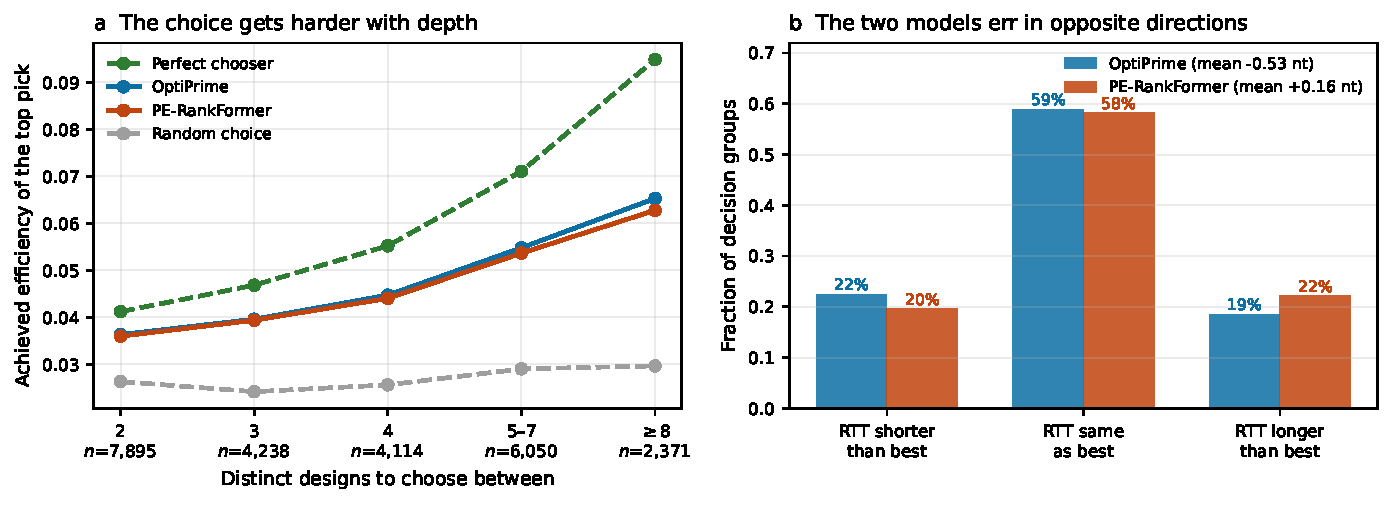
\includegraphics[width=\textwidth]{figures_explore_v2/fig_decision.pdf}
\caption{\textbf{Where the deficit lives.} \textbf{(a)}~Achieved efficiency of the top pick
against the number of distinct designs the user is choosing between, on the reserved panel.
At a binary choice the two models are indistinguishable; the gap opens as the choice gets
harder, which is where a ranking model earns its keep. Both stay far above random selection
and far below a perfect chooser. \textbf{(b)}~Direction of the error in RTT length. Where a
model does not nominate the best-measured design, OptiPrime errs towards shorter RTTs and
PE-RankFormer towards longer ones. The models fail in opposite directions, not by different
amounts. \S\ref{sec:blend} shows this is exploitable: an equal-weight average of the two
scores beats both.}
\label{fig:decision}
\end{figure}

\subsection{How large is the disagreement?}

% generated by explore_v2/make_report_tables.py -- do not edit by hand
\begin{table}[htbp]\centering\begin{threeparttable}
\caption{Where the decision is lost. On 24,668 informative panel groups a random pick achieves
0.0268 and a perfect chooser 0.0570, so the whole decision is worth 0.0302 efficiency. Length bias
is the mean difference in PBS or RTT length between the design a model nominates and the
best-measured design.}
\label{tab:geometry}\footnotesize
\begin{tabular}{l S[table-format=1.4] S[table-format=2.1] S[table-format=+1.3] S[table-format=+1.3]}
\toprule
Model & {Achieved @1} & {\% of gain} & {PBS bias} & {RTT bias} \\
\midrule
OptiPrime & 0.0456 & 62.2 & +0.519 & -0.531 \\
PE-RankFormer (published) & 0.0448 & 59.6 & +0.766 & +0.162 \\
Arm A, 3 seeds (released) & 0.0431 & 54.1 & +0.943 & +0.483 \\
Arm F, 3 seeds & 0.0446 & 58.9 & +0.812 & +0.428 \\
\bottomrule
\end{tabular}

\vspace{0.9em}
\begin{tabular}{lrrrrrrrr}
\toprule
$\alpha$ & $-0.010$ & $-0.006$ & $-0.004$ & $-0.002$ & $-0.001$ & $+0.000$ & $+0.001$ & $+0.002$ \\
\midrule
Achieved @1 & 0.28703 & 0.28987 & 0.29080 & 0.29168 & 0.29213 & 0.29213 & 0.29183 & 0.29118 \\
\bottomrule
\end{tabular}
\begin{tablenotes}[flushleft]\footnotesize
\item The sweep adds $\alpha\cdot\mathrm{len(RTT)}$ to the out-of-fold score on 43,425
development decision groups against a baseline of 0.29213. The optimum is exactly $\alpha=0$:
the length preference is not a global additive offset and cannot be removed by one.
\end{tablenotes}\end{threeparttable}\end{table}


A difference at the fourth decimal place of an efficiency is hard to interpret directly. The
informative denominator is the gain a perfect chooser would deliver over a random one. On that
scale both models capture most of what is available and the difference between them is 2.6\%
of it. We recommend stating the comparison in these units in either direction: the deficit is
statistically unambiguous and practically small, and a reader deserves both facts.

\subsection{Why two defensible metrics disagree}

Pooled correlation and the fixed-allele decision are different estimands measured on the same
rows. The first asks how well the entire list is ordered and mixes ``which locus and condition
is easy'' with ``which design is best''; the second isolates the latter by construction. They
need not agree, and here they do not.

The disagreement is not an artefact of comparing across model families. It reproduces between
two of our own published members, which differ only in their output head. On the panel the
ordinal head wins the decision by $0.00026$ ($p = 0.009$), while pooled $\rho$ prefers the
simplex head, 0.7126 against 0.7091. The same two numbers, computed on the same rows of the
same two checkpoints, would justify shipping either architecture depending on which metric
the paper had nominated as its headline. That is a reason to fix the estimand before
measuring, not after.

% =====================================================================
\section{Improving the model}

\subsection{An eight-arm training matrix}
\label{sec:matrix}

% generated by explore_v2/make_report_tables.py -- do not edit by hand
\begin{table}[htbp]\centering\begin{threeparttable}
\caption{The decision-aligned training matrix, scored on fold 0's 1,463 informative decision
groups. No arm trains or early-stops on fold 0.}
\label{tab:matrix}\footnotesize
\begin{tabular}{cl S[table-format=1] S[table-format=1.5] S[table-format=1.4] S[table-format=6.0]}
\toprule
Arm & What it changes & {Seeds} & {Achieved @1} & {Pooled $\rho$} & {Pairs/epoch} \\
\midrule
A & original batching, original ranking key & 3 & 0.13360 & 0.8905 & 15695 \\
B & canonical batching, original ranking key & 1 & 0.13205 & 0.8703 & 6975 \\
C & canonical both, 1 pair per group & 1 & 0.13463 & 0.8950 & 25253 \\
D & canonical batching, canonical ranking key & 3 & 0.13453 & 0.8950 & 61978 \\
E & canonical batching, ranking disabled & 3 & 0.13459 & 0.8949 & 61975 \\
F & canonical both, feature branch & 3 & 0.13523 & 0.8974 & 61976 \\
G & canonical both, 16 pairs per group & 1 & 0.13357 & 0.8968 & 146088 \\
H & canonical batching, feature branch, ranking disabled & 3 & 0.13473 & 0.8971 & 61976 \\
\bottomrule
\end{tabular}

\vspace{0.9em}
\begin{tabular}{l S[table-format=1] S[table-format=+1.5] l}
\toprule
Seed-paired contrast & {Seeds} & {Mean $\Delta$} & {All seeds agree in sign} \\
\midrule
F $-$ A & 3 & +0.00164 & yes \\
E $-$ A & 3 & +0.00099 & yes \\
H $-$ A & 3 & +0.00114 & yes \\
D $-$ A & 3 & +0.00093 & yes \\
F $-$ E & 3 & +0.00064 & yes \\
H $-$ F & 3 & -0.00050 & yes \\
F $-$ D & 3 & +0.00071 & \textbf{no} \\
D $-$ E & 3 & -0.00006 & \textbf{no} \\
H $-$ E & 3 & +0.00014 & \textbf{no} \\
D $-$ C & 1 & -0.00008 & {--} \\
G $-$ D & 1 & -0.00098 & {--} \\
B $-$ A & 1 & -0.00197 & {--} \\
D $-$ B & 1 & +0.00250 & {--} \\
\bottomrule
\end{tabular}
\begin{tablenotes}[flushleft]\footnotesize
\item A contrast whose seeds disagree in sign is not evidence for a mechanism however large
its mean. On that criterion the load-bearing effects here are canonical batching (E $-$ A)
and the feature branch (F $-$ E), while the ranking-pair contrast with batching held fixed
(D $-$ E) is not one of them. \textbf{Only the first of those survives an external library:}
on the reserved panel F $-$ E reverses sign to $-0.00025$ ($p = 0.006$), so three-of-three
seed agreement on the held-out fold did not make it a safe component decision
(Table~\ref{tab:armspanel}).
\item \textbf{Checkpoint selection is a null.} Selecting on the decision metric rather than
pooled $\rho$ gains +0.00004 in fold-0 achieved efficiency over the same 18 trajectories,
even though the two selectors choose different epochs in 16 of them.
\end{tablenotes}\end{threeparttable}\end{table}


Regrouping the training key changes two things at once: which rows share a \emph{batch}, and
which rows can form a \emph{ranking pair}. Our earlier claim was that the gain came from
ranking-pair exposure --- letting the pairwise objective see comparisons it had been blind to.
The matrix separates the two, and refutes that claim.

Arm E disables the ranking loss entirely and still captures 60\% of the total gain. The
contrast that isolates pair exposure with batching held fixed, D $-$ E, is $-0.00006$ and
flips sign across seeds. Arm G, which raises the pair budget to sixteen per group and
2.4$\times$ arm D's pairs per epoch, is \emph{worse} than arm D. The mechanism is batch
composition: grouping comparable candidates into the same batch changes the gradient through
batch statistics whether or not they are subsequently formed into pairs. We withdraw the
exposure claim. On this surface the batching effect and the feature branch survive as the two
seed-stable gains --- but \S\ref{sec:armspanel} shows that only the first of them survives an
external library, which is the reason this section is not the end of the argument.

\subsection{Two things the matrix rules out}

Checkpoint selection is a null (Table~\ref{tab:matrix}, note). And a per-candidate score
correction cannot fix the residual error: sweeping a linear length term over 43{,}425
development decision groups, the optimum is exactly zero on both the PBS and RTT axes
(Table~\ref{tab:geometry}). Since the length preference is real but not a global offset, it
must be conditional on allele and context --- which is an argument for scoring the candidate
set jointly rather than each candidate independently.

\subsection{Which parts of the recipe survive an external library}
\label{sec:armspanel}

% generated by explore_v2/make_report_tables.py -- do not edit by hand
\begin{table}[htbp]\centering\begin{threeparttable}
\caption{Every training arm's three-seed ensemble on the reserved panel, all eligible groups.
Ensemble size is matched across arms, so it cannot explain a difference, and feature
standardisation is frozen to each checkpoint's training folds. Arms marked $\dagger$ carry the
Family C feature branch.}
\label{tab:armspanel}\scriptsize
\begin{tabular}{@{}ll S[table-format=1.4] S[table-format=1.4]
                    S[table-format=+1.5] S[table-format=+1.5] l@{}}
\toprule
& & & & \multicolumn{2}{c}{$\Delta$ achieved @1 vs.} & \\
\cmidrule(lr){5-6}
Arm & What it changes & {Achieved @1} & {Pooled $\rho$} & {OptiPrime} & {published} & {$p$} \\
\midrule
A & released recipe & 0.0349 & 0.6908 & -0.00198 & -0.00134 & 0.001 \\
D & canonical batching, ranking on & 0.0362 & 0.7019 & -0.00070 & -0.00006 & 0.517 \\
E & canonical batching, ranking off & 0.0363 & 0.7070 & -0.00057 & +0.00006 & 0.464 \\
F$\dagger$ & canonical batching, ranking on & 0.0361 & 0.7071 & -0.00083 & -0.00019 & 0.044 \\
H$\dagger$ & canonical batching, ranking off & 0.0365 & 0.7113 & -0.00040 & +0.00024 & 0.020 \\
\midrule
OptiPrime & & 0.0369 & 0.6931 & & & \\
PE-RankFormer (published) & & 0.0363 & 0.7091 & & & \\
\bottomrule
\end{tabular}
\begin{tablenotes}[flushleft]\footnotesize
\item The $p$ column refers to the contrast against the published member. Ten contrasts were
computed on this surface, so a nominal $p$ near 0.02 is weak evidence; and the panel is used
here for development, not confirmation.
\end{tablenotes}\end{threeparttable}\end{table}


The fold-0 matrix nominated arm F. Scoring every arm on the panel --- ensemble size matched
at three seeds, feature standardisation frozen --- shows that only part of the fold-0 story
transfers, and one part of it inverts.

\paragraph{Canonical batching transfers, and it is the whole gain.}
$\mathrm{E}-\mathrm{A} = +0.00141$ ($p = 0.001$): arm E, which changes nothing but which rows
share a batch and switches the ranking loss \emph{off}, captures the entire improvement over
the released recipe and draws level with the published model ($+0.00006$, $p = 0.46$). This
is the fold-0 conclusion confirmed on an external library.

\paragraph{The ranking loss costs accuracy here.}
Comparing the arms that differ only in whether the pairwise term is active: with the feature
branch on, $\mathrm{H}-\mathrm{F} = +0.00043$; without it,
$\mathrm{E}-\mathrm{D} = +0.00010$. Both favour switching it off, and so does pooled $\rho$
(0.7113 against 0.7071 with features; 0.7070 against 0.7019 without). On 30{,}475 panel
groups the pairwise objective is a consistent small cost on \emph{both} metrics --- a rare
case in this programme of the two estimands agreeing.

\paragraph{Two ablation conclusions that did not transfer.}
Fold 0 said the opposite, and said it with the evidence standard this project had been using.

\begin{center}\footnotesize
\begin{tabular}{lS[table-format=+1.5]cS[table-format=+1.5]c}
\toprule
& \multicolumn{2}{c}{held-out fold 0} & \multicolumn{2}{c}{reserved panel} \\
\cmidrule(lr){2-3}\cmidrule(lr){4-5}
Contrast & {mean $\Delta$} & seeds agree & {mean $\Delta$} & $p$ \\
\midrule
F $-$ E \quad\emph{(add ranking + features)} & +0.00064 & 3/3 & -0.00025 & 0.006 \\
H $-$ F \quad\emph{(drop ranking, features on)} & -0.00050 & 3/3 & +0.00043 & {--} \\
\bottomrule
\end{tabular}
\end{center}

\noindent Both reverse sign, and on fold 0 both had all three seeds agreeing. We had treated
three-of-three sign agreement on the held-out fold as sufficient evidence for a component
decision. These are measured counterexamples, and they are the strongest practical argument
in this report for validating ablation choices on a surface the development corpus did not
choose. Seed agreement measures optimisation noise; it says nothing about transfer.

\paragraph{The feature branch is roughly neutral, not a liability.}
Isolated with the ranking loss off, $\mathrm{H}-\mathrm{E} = +0.00018$ ($p = 0.068$). Our
prior reading --- that the branch extrapolates badly on a shifted library and costs accuracy
--- is not supported. What the frozen-standardisation fix (\S\ref{sec:corrections}) actually
removed was an artefact that had \emph{flattered} the branch; with it gone the branch is
close to doing nothing, and the arm that carries it and drops the ranking loss (H) is the
best configuration we found.

\paragraph{What we may and may not conclude from this.}
Arm H beats the published member on the decision ($+0.00024$, $p = 0.020$) and on pooled
$\rho$ (0.7113 against 0.7091), and it has the smallest deficit to OptiPrime of any arm
($-0.00040$). We are \emph{not} entitled to call that a result. It was found by scoring ten
contrasts on the panel, so a nominal $p = 0.020$ is weak; the panel is being used for
development here, not confirmation; and adopting arm H now would be selecting a component on
the very surface used to evaluate it --- the error this report criticises elsewhere. The
defensible statement is that the pre-specified fold-0 selection chose arm F, the panel
suggests that choice was wrong in a specific and mechanistically interpretable way, and
testing arm H properly requires a freshly reserved surface.

\subsection{The recipe, built the way the published model is built}
\label{sec:perfold}

Everything in \S\ref{sec:armspanel} compares three-seed ensembles, and the published model is
not one. It is five checkpoints, one per official fold, each trained on a different
four-fifths of the development data. Three seeds trained on identical rows differ only in
initialisation and are a far less diverse ensemble, so every contrast against the published
member above confounds recipe with ensemble construction.

This removes that confound: arm F rebuilt as five per-fold checkpoints, combined by the same
plain mean of predicted efficiencies used to form the published member, with the isotonic
calibrator refitted from scratch on \emph{this} model's development out-of-fold predictions
and frozen before either surface was touched. Fold 0 is the official test fold and no member
trains or early-stops on it.

Arm F is the right arm to build this way even though \S\ref{sec:armspanel} suggests arms E
and H are ahead of it on the panel, because arm F is what the pre-specified fold-0 selection
chose. Building the arm the panel prefers would be selecting on the evaluation surface.

% generated by explore_v2/make_report_tables.py -- do not edit by hand
\begin{table}[htbp]\centering\begin{threeparttable}
\caption{Does the improved recipe beat the published model when the two are built alike?
Both are five checkpoints, one per official fold, combined by the same plain mean of
predicted efficiencies. Achieved efficiency at rank 1, all eligible panel groups.}
\label{tab:headline}\scriptsize
\begin{tabular}{l S[table-format=+1.5] l l}
\toprule
Contrast & {$\Delta$ achieved @1} & {95\% CI} & {$p$} \\
\midrule
\textbf{Arm F, 5 per-fold} $-$ PE-RankFormer (published) & -0.00017 & $[-0.00034,\,+0.00001]$ & 0.062 \\
\textbf{Arm F, 5 per-fold} $-$ Arm F, 3 seeds & +0.00002 & $[-0.00015,\,+0.00020]$ & 0.812 \\
\textbf{Arm F, 5 per-fold} $-$ Arm A, 3 seeds (released) & +0.00117 & $[+0.00095,\,+0.00140]$ & 0.001 \\
\textbf{Arm F, 5 per-fold} $-$ Arm E, 3 seeds & -0.00023 & $[-0.00043,\,-0.00004]$ & 0.014 \\
\textbf{Arm F, 5 per-fold} $-$ Arm H, 3 seeds & -0.00041 & $[-0.00059,\,-0.00023]$ & 0.001 \\
\textbf{Arm F, 5 per-fold} $-$ OptiPrime & -0.00081 & $[-0.00107,\,-0.00055]$ & 0.001 \\
PE-RankFormer (published) $-$ OptiPrime & -0.00064 & $[-0.00089,\,-0.00038]$ & 0.001 \\
\quad on fold 0: \textbf{Arm F, 5 per-fold} $-$ PE-RankFormer (published) & +0.00007 & $[-0.00152,\,+0.00173]$ & 0.952 \\
\quad on fold 0: \textbf{Arm F, 5 per-fold} $-$ OptiPrime & +0.00922 & $[+0.00612,\,+0.01255]$ & 0.001 \\
\bottomrule
\end{tabular}\end{threeparttable}\end{table}


\paragraph{The ensemble-construction hypothesis is refuted.}
Building arm F as five per-fold checkpoints instead of three same-data seeds changes
essentially nothing: $+0.00002$ ($p = 0.81$). Whatever explains arm F's failure to overtake
the published member, it is not that the two were built differently. E22's conjecture was
wrong.

\paragraph{The improved recipe does not beat the published model.}
$-0.00017$ on the panel with an interval spanning zero ($[-0.00034, +0.00001]$, $p = 0.062$),
and $+0.00007$ on fold 0 ($p = 0.95$). Pooled $\rho$ is likewise indistinguishable: 0.7096
against 0.7091 on the panel, 0.9084 against 0.9079 on fold 0. Two surfaces, two metrics, no
difference. It also remains behind OptiPrime on the panel decision ($-0.00081$, $p = 0.001$)
and behind arms E and H, consistent with \S\ref{sec:armspanel}.

\paragraph{An unexplained gap that bounds what the matrix can claim.}
Arm A is our reconstruction of the released recipe, and it scores 0.0349 on the panel against
the published member's 0.0363 --- a gap of 0.00135, larger than any effect in the ablation
matrix. Per-fold construction cannot explain it, because we have just measured that as worth
$+0.00002$. So arm A is not a faithful reproduction of the published model, and every
improvement the matrix reports is an improvement over \emph{our reconstruction}, not over the
shipped system. Arm F's $+0.00117$ over arm A is real and replicates; it simply lands the
model back where the published member already was.

This is the honest close to the recipe question. The matrix found a training change that is
reproducible, seed-stable on the development fold, and worth about a tenth of a percent of
achieved efficiency over our own baseline --- and that nonetheless leaves the shipped model
exactly where it was. The gain the manuscript could claim from it is zero.

% =====================================================================
\section{Diagnosis of the residual error}

On the groups where the two models nominate different designs, the nominated designs differ
systematically in geometry (Table~\ref{tab:geometry} and Figure~\ref{fig:decision}b). Every
PE-RankFormer variant prefers a
longer PBS \emph{and} a longer RTT than the best-measured design. OptiPrime is the only model
that prefers a shorter RTT, which is consistent with its treating RTT length as an explicit
repeat count in a synthesis rate term --- a structural prior our architecture lacks. The
engineered-feature branch supplies PBS and RTT lengths to the network as explicit scalars. It
moves the PBS bias by $-0.131$ and the RTT bias by $-0.055$: both shrink a little, neither is
removed, and both remain on the opposite side of zero from OptiPrime. Handing the model the
length is evidently not the same as modelling what the length does.

Freezing feature standardisation to each checkpoint's training statistics
(\S\ref{sec:corrections}) sharpened this picture. Panel \code{pbs\_length} sits 1.35 training
SDs below the training mean with twice the spread, so at deployment the branch reads inputs
well outside the range it was fitted on, and refitting the statistics on the panel had been
concealing that. Scored honestly, arm F's advantage over the released recipe falls from
$+0.00140$ to $+0.00115$.

Our first reading of that was that the branch extrapolates badly and costs accuracy on a
shifted library. Isolating it properly (\S\ref{sec:armspanel}) does not support this: with
the ranking loss held off, adding the branch is worth $+0.00018$ ($p = 0.068$). The branch is
close to inert on this surface. What the correction removed was an artefact that had
\emph{flattered} it, not evidence that it hurts --- and an evaluation that restandardises on
the test surface would have reported the flattering number.

\subsection{A practical consequence, and its boundary}
\label{sec:blend}

If the two models err in opposite directions, their errors may partly cancel. That is an
empirical question the bias table cannot settle, so we tested it: an equal-weight rank
average of the two scores. The weight is fixed at one half and nothing is fitted.

\begin{table}[htbp]\centering\begin{threeparttable}\footnotesize
\caption{An equal-weight rank average of OptiPrime and PE-RankFormer, on both surfaces.
Intervals are cluster bootstraps resampling target sites.}
\label{tab:blend}
\begin{tabular}{l S[table-format=1.4] S[table-format=+1.5] l l}
\toprule
Model & {Achieved @1} & {$\Delta$ vs.\ blend} & {95\% CI} & {$p$} \\
\midrule
\multicolumn{5}{l}{\emph{reserved panel --- 24,668 informative groups}}\\[1pt]
OptiPrime & 0.0456 & -0.00055 & $[-0.00077,\,-0.00034]$ & $<$0.001 \\
PE-RankFormer (published) & 0.0448 & -0.00133 & $[-0.00156,\,-0.00109]$ & $<$0.001 \\
\textbf{Equal-weight rank average} & \bfseries 0.0461 & {--} & & \\
\midrule
\multicolumn{5}{l}{\emph{held-out fold 0 --- 1,463 informative groups}}\\[1pt]
OptiPrime & 0.1272 & -0.00429 & $[-0.00615,\,-0.00257]$ & $<$0.001 \\
\textbf{PE-RankFormer (published)} & \bfseries 0.1364 & +0.00486 & $[+0.00278,\,+0.00704]$ & $<$0.001 \\
Equal-weight rank average & 0.1315 & {--} & & \\
\bottomrule
\end{tabular}
\begin{tablenotes}[flushleft]\footnotesize
\item Fold 0 is a legitimate second surface for this particular claim: no parameter is
fitted here either, so evaluating on it costs nothing that was being reserved.
\end{tablenotes}\end{threeparttable}\end{table}

\paragraph{On the panel the blend wins, and not by a lucky weight.}
It captures 64.1\% of the gain a perfect chooser would deliver, against 62.2\% for OptiPrime
alone, and it beats the better of the two by more than PE-RankFormer trails it. Sweeping the
weight on PE-RankFormer from 0 to 1, \emph{every} intermediate value from 0.2 to 0.7 beats
both endpoints (0.04589, 0.04607, 0.04607, 0.04614, 0.04597, 0.04576 against 0.04559 for
OptiPrime alone and 0.04481 for PE-RankFormer alone). The equal-weight choice is not
cherry-picked.

\paragraph{On fold 0 it does not, and that is informative rather than fatal.}
There the blend beats OptiPrime by $+0.00429$ but \emph{loses} to PE-RankFormer alone by
$0.00486$. The reason is visible in the numbers: on fold 0 PE-RankFormer leads OptiPrime by
0.0092, a wide margin, so averaging in the weaker model dilutes the stronger one. On the
panel the two are within 0.0008 of each other and the blend pays. Blending helps when the
components are comparably strong, which is the ordinary behaviour of ensembles and not a
special property of these two models.

\paragraph{What we therefore claim.}
Not that the blend is universally better. The defensible statement is narrower and still
useful: \emph{on the surface that resembles deployment} --- an external library, realistic
candidate depth, the two models within a thousandth of each other --- combining them beats
either alone, robustly across weights, with nothing fitted. And the mechanism is the one
Figure~\ref{fig:decision}b shows, not generic ensembling: the two models disagree about RTT
geometry in opposite directions. That is an argument for treating the mechanistic baseline as
complementary to the neural model rather than as a rival to be beaten.

% =====================================================================
\section{Corrections to this programme's own work}
\label{sec:corrections}

A re-evaluation that finds errors in others' work should be held to the same standard.
\code{explore\_v2/CORRECTIONS.md} records every correction; the load-bearing ones are:

\begin{itemize}\itemsep3pt
\item \textbf{A strand-invariance bug in the canonical key.} Left-normalisation was applied on
the forward strand and the result reverse-complemented, so an indel could key differently
depending on the orientation it was reported in; 61.7\% of 51{,}012 indel pairs were exposed.
Fixed by normalising each orientation independently. Fold-0 group counts were unchanged.
\item \textbf{The exposure claim, withdrawn} (\S\ref{sec:armspanel}), after three-seed
replication showed that the contrast it rested on flips sign.
\item \textbf{Two index-mapping bugs} in the exposure replay: sampler indices are into the
training subset, not the corpus. These produced an impossible statistic (100\% of canonical
pairs spanning two alleles) and a negative mean target gap where the minimum is $0.02$.
\item \textbf{A per-epoch decision metric that assumed sorted rows.} A \code{reduceat} over an
unsorted group column invented 14{,}680 boundaries against 11{,}559 real groups. After fixing,
the vectorised arithmetic was validated against a brute-force per-group loop --- exact match.
\item \textbf{Feature standardisation refit on the evaluation surface.} The Family C feature
statistics are recomputed at attach time and are not stored in the checkpoint, so scoring a new
surface silently restandardised the inputs by that surface's own mean and SD. On the panel this
is not cosmetic: \code{pbs\_length} sits 1.35 training SDs low with twice the spread, and
\code{pbs\_tm} 0.86 SDs low with 2.2$\times$ the spread. Fixed by freezing each checkpoint's
training statistics (\code{explore\_v2/featstats.py}) and re-scoring.
\item \textbf{Two readings we formed and then withdrew in the course of this report.}
First, that the feature branch extrapolates badly on a shifted library and costs accuracy;
isolating it properly gives $+0.00018$ ($p = 0.068$), close to inert
(\S\ref{sec:armspanel}). Second, that the equal-weight blend beats both models; it does on
the panel but loses to PE-RankFormer alone on fold 0 (\S\ref{sec:blend}). Both were formed
from one surface before the second had been looked at, which is the error this report
attributes to others; both are stated here with the evidence that overturned them rather
than quietly revised.

\item \textbf{A verifier that double-counted its own claims.} The claim list had accumulated
six partial copies of one block; 268 registered claims were 133 distinct ones, three of which
still carried single-seed values superseded by the reseeded matrix. Fifty-six further claims
were added to cover E18 and E22--E24 and the grouping figures quoted in \S2, giving the 188
checked today.
\end{itemize}

% =====================================================================
\section{Limits}

\begin{itemize}\itemsep3pt
\item \textbf{One reserved surface, spent once.} Only the E11/E16 comparison is confirmatory.
Every other panel result here is development work.
\item \textbf{One library, one laboratory, HEK293T-dominated.} The panel does not test
cross-cell-type or cross-editor generalisation.
\item \textbf{Bounded by what was measured.} Achieved efficiency is scored against the best
\emph{measured} design in a group, not the best designable one.
\item \textbf{Our baseline is not the shipped model.} Arm A, the reconstruction every
ablation contrast is measured against, sits 0.00135 below the published member on the panel
--- more than any effect the matrix reports, and not explained by ensemble construction
(\S\ref{sec:perfold}). Training-recipe conclusions in \S\ref{sec:matrix}--\S\ref{sec:perfold}
are therefore relative to that reconstruction, and the difference between it and the released
system is unaccounted for.

\item \textbf{No wet-lab validation.} Every claim here is retrospective.
\item \textbf{Small effects.} The programme's resolution on fold 0 is about 0.005 in pooled
$\rho$; the decision differences separating methods are an order of magnitude smaller, which
is why 24{,}668 panel groups were needed to see them at all.
\end{itemize}

% =====================================================================
\section{Recommendations}

These are ordered by how much they change what the manuscript asserts. Line references are to
\code{reports/paper/pe\_rankformer\_paper.tex}.

\begin{enumerate}\itemsep4pt
\item \textbf{Stop calling the within-protospacer evaluation ``the deployment-relevant task''}
(l.~55, and again in the utility section at l.~757, ``computed within a protospacer
group'').
That grouping is not the decision a user faces: all 670 of its groups span more than one
source/cell/editor condition and 26\% contain more than one intended allele, so a ranking
inside one mixes which condition is easy with which design is best. The deployment unit is
one canonical allele in one context. This is the single most consequential change, because
the sentence currently claims the very thing the corrected estimand reverses.

\item \textbf{Withdraw the implied deployment-superiority claim and state the sized
comparison.} Under the correct grouping, on a library neither model trained on, OptiPrime
obtains more efficiency from its top pick. Report it in interpretable units: OptiPrime
captures 62.2\% of the gain a perfect chooser would deliver and PE-RankFormer 59.6\%, a
difference of 2.6\% of what is available, with both models far above random selection.

\item \textbf{Correct the row-versus-design accounting} behind the ``735 targets with five or
more designs'' population. Those groups contain five or more \emph{rows}; their median
distinct-design count is two, and under the correct grouping fold 0 contains \emph{no} group
with five distinct designs. Any ``best of five'' endpoint computed on fold 0 should be
withdrawn or recomputed on the panel.

\item \textbf{Promote the metric disagreement from a caveat to a finding.} The manuscript
already says the ranking and outcome metrics disagree (l.~759, ``the disagreement is the
result''), which is the right instinct --- but it reports the disagreement in magnitude only.
Under the corrected grouping the disagreement is in \emph{sign}, it reproduces inside our own
ablations (the ordinal head wins the decision at $p = 0.009$ while pooled $\rho$ prefers the
simplex head), and that is a more general and more useful claim than the margin it replaces.

\item \textbf{Report the ablation matrix with its withdrawn claim intact.} Batch composition,
not ranking supervision, is what pays; the contrast that isolates ranking-pair exposure is
$-0.00006$ and flips sign across seeds. Reporting the correction is what makes the surviving
effects credible.

\item \textbf{Validate component choices outside the development corpus before shipping
them.} $\mathrm{F}-\mathrm{E}$ was $+0.00064$ on the held-out fold with all three seeds
agreeing in sign --- the evidence standard this project had been using --- and it is
$-0.00025$ ($p = 0.006$) on an external library. Seed agreement measures optimisation noise,
not transfer. Any component the paper claims as a contribution should be shown to survive a
surface the development corpus did not choose.

\item \textbf{Report the blend, with its boundary.} On the panel an equal-weight rank
average of PE-RankFormer and OptiPrime beats both ($+0.00055$ over OptiPrime, $p<0.001$),
with nothing fitted and robustly across weights; on fold 0, where PE-RankFormer dominates, it
does not. Reported together these say something useful: the mechanistic baseline is
complementary to the neural model wherever the two are comparably strong, which is the
regime an external library puts them in. That is better supported than a superiority claim in
either direction.

\item \textbf{Freeze feature standardisation at the checkpoint and say so.} The released
scoring path refits Family C statistics on whatever data it is handed, silently
restandardising any new library by its own mean and SD. This is a correctness fix with a
reporting consequence: an evaluation done that way quotes a better number than the model
would deliver, because it erases the distribution shift the evaluation exists to measure.
\end{enumerate}

\section*{Reproducibility}

Scripts, JSON artifacts and Markdown reports for E01--E24 are in \code{explore\_v2/}. Endpoint
invariants: \code{explore\_v2/test\_endpoints.py} (13 tests). Numeric claims:
\code{explore\_v2/verify\_report.py} (188 claims). Tables in this report are generated by
\code{explore\_v2/make\_report\_tables.py} directly from the JSON artifacts, so the report
cannot drift from the data.

\end{document}
